\subsubsection{Settimo periodo (2024/03/07 - 2024/03/24)}

\subsubsubsection{Planning}
%Il gruppo \emph{Ramtastic6} ha deciso di pianificare uno $\textit{sprint}_G$ breve della durata di una settimana per raggiungere risultati per obiettivi ben definiti e significativi seppur di durata per il loro raggiungimento contenuta.


\subsubsubsubsection*{Attività pianificate}
All'inizio del periodo ad ogni membro del gruppo sono stati assegnati ruoli specifici, di seguito riportati:
\begin{table}[H]
\centering
\begin{tabular}{|c|c|c|}
\hline
\textbf{Membro} & \textbf{Ruolo} \\
\hline
Samuele V. & Programmatore \\
\hline
Michele Z. & Programmatore \\
\hline
Leonardo B. & Amministratore \\
\hline
Riccardo Z. & Responsabile \\
\hline
Filippo T. & Programmatore \\
\hline
Davide B. & Analista \\
\hline
\end{tabular}
\caption{Ruoli assunti per ciascun membro del team all'inizio del periodo}
\end{table}

Gli obiettivi posti per lo $\textit{sprint}_G$ sono stati i seguenti:
\begin{itemize}
    \item Per quanto riguarda il \emph{PoC}:
    \begin{enumerate}
        \item Approfondire ulteriormente le $\textit{tecnologie}_G$ individuate per la sua realizzazione come Next js, Nest js e $\textit{Docker}_G$ e contestualmente rivedere l'organizzazione del $\textit{repository}_G$ per lo sviluppo.
        \item Raggiungere una configurazione accettabile per il \emph{PoC};
        \item Creare una prima versione del database (lato back-end);
        \item Raggiungere una prima implementazione della funzionalità di ricerca dei ristoranti (lato back-end e front-end);
        \item Chiedere $\textit{feedback}_G$ al proponente riguardo la configurazione raggiunta e consigli per quanto riguarda la $\textit{feature}_G$ di $\textit{ordinazione}_G$.
    \end{enumerate}
    \item Aggiornare \emph{Piano di Progetto} riportando gli $\textit{sprint}_G$ mancanti e i nuovi $\textit{sprint}_G$;
    \item Redigere una prima versione del documento \emph{Piano di Qualifica};
    \item Completare l'automazione e la stesura di una prima versione del glossario;
    \item Completare la pagina $\textit{github}_G$.io riguardante il sunto dei documenti nel $\textit{repository}_G$ \emph{RAMtastic6.$\textit{github}_G$.io}, completare l'automazione inerente e inserirla nello stesso $\textit{repository}_G$;
    \item Esplorare le potenzialità di $\textit{jira}_G$ per analizzare il lavoro fatto.
\end{itemize}

\subsubsubsubsection*{Preventivo}
\begin{table}[H]
    \centering
\begin{spreadtab}{{tabular}{|c|c|c|c|c|c|c|c|}}
    \hline
    @\textbf{Membro} & @\textbf{Re} & @\textbf{Amm} & @\textbf{An} & @\textbf{Progr} & @\textbf{Proge} & @\textbf{Ve} & @\textbf{Totale} \\
    \hline
    @ Samuele V.   & 0          & 0          & 0        & 6.5          & 0     & 1     & sum(b2:g2) \\
    @ Leonardo B.  & 0         & 5          & 0        & 0        & 0     & 1    & sum(b3:g3) \\
    @ Riccardo Z.  & 6          & 3          & 0          & 2          & 0     & 1   & sum(b4:g4) \\
    @ Davide B.    & 0          & 1          & 2      & 0       & 0     & 4.5     & sum(b5:g5) \\
    @ Michele Z.   & 0          & 1          & 0         & 2          & 0     & 0     & sum(b6:g6) \\
    @ Filippo T.   & 0          & 0          & 0         & 5          & 0     & 0     & sum(b7:g7) \\
    \hline
    @\textbf{Ore totali} & sum(b2:b7) & sum(c2:c7) & sum(d2:d7) & sum(e2:e7) & sum(f2:f7) & sum(g2:g7) &  sum(b8:g8)\\
    \hline
    @\textbf{Costo totale} & 30*b8 & 20*c8 & 25*d8 & 15*e8 & 25*f8 & 15*g8 & sum(b9:g9)\\
    \hline
\end{spreadtab}
    \caption{Consuntivo orario ed economico parziale per il settimo periodo, in base al ruolo}
    \label{tab:prev_rtb}
    \vspace{5mm}
    \textbf{Legenda:} \textit{Re} = Responsabile, \textit{Amm} = Amministratore, \textit{An} = Analista, \textit{Progr} = Programmatore, \textit{Proge} = Progettista, \textit{Ve} = Verificatore
\end{table}
\begin{figure}[H]
  \centering
  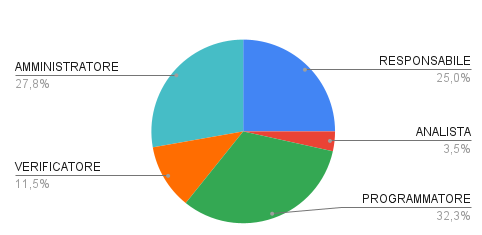
\includegraphics[width=0.6\linewidth]{grafici/7_periodo_torta.png}
  \caption{Ripartizione dei costi per ruolo nel $7^\circ$ periodo}
        \vspace{10mm}
  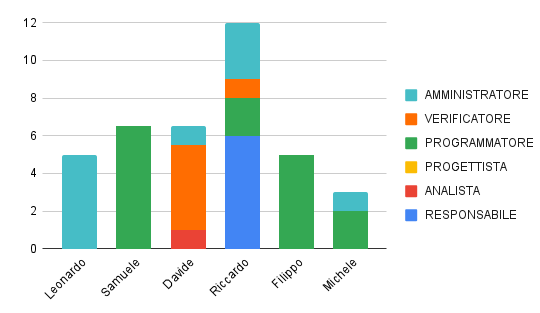
\includegraphics[width=0.7\linewidth]{grafici/7_periodo_istogramma.png}
  \caption{Ore preventivate per ciascuna persona nel $7^\circ$ periodo}
\end{figure}
\subsubsubsection{Review}
\subsubsubsubsection*{Attività svolte}
Le attività previste sono state svolte con relativo successo, in particolare:
\begin{itemize}
    \item Per quanto riguarda il \emph{PoC}:
    \begin{enumerate}
        \item I programmatori coinvolti si sono allineati sulle $\textit{tecnologie}_G$;
        \item E' stata raggiunta una configurazione accettabile per il suo sviluppo;
        \item E' stata implementata una prima versione della funzionalità di ricerca dei ristoranti con la nuova configurazione (lato back-end e front-end).
    \end{enumerate}
    \item \emph{Piano di Progetto} è stato aggiornato come previsto;
    \item \emph{Piano di Qualifica} è stato iniziato come previsto;
    \item L'automazione per generare il glossario tecnico è stata completata;
    \item Una prima versione della pagina $\textit{github}_G$.io; è stata completata l'automazione atta a generarla ed è stata inserita nel $\textit{repository}_G$ \emph{RAMtastic6.$\textit{github}_G$.io};
    \item L'organizzazione del \emph{PoC} e del $\textit{way of working}_G$ è stata rivista come riportato nel $\textit{verbale}_G$ del 13/03/2024;
    \item Le potenzialità di $\textit{jira}_G$ sono state esplorate al fine di garantire una miglior collaborazione come riportato nel $\textit{verbale}_G$ del 13/03/2024;
    \item E' stato effettuato un incontro con il proponente in data 21/03/2024. In particolare:
    \begin{itemize}
        \item E' stato fornito un $\textit{feedback}_G$ positivo riguardante l'utilizzo dei file \emph{Json} e delle \emph{API rest} come mezzo di comunicazione tra \emph{NextJs} e \emph{NestJs}
        \item E' stato consigliato l'uso dei \emph{custom hooks};
        \item Sono stati forniti dei consigli per quanto riguarda la realizzazione della $\textit{feature}_G$ dell'$\textit{ordinazione}_G$ collaborativa. In questo contesto stato introdotto brevemente il concetto di \emph{socket};
        \item Sono stati chiariti dubbi riguardanti il ruolo del \emph{project manager}.
    \end{itemize}
\end{itemize}
\subsubsubsubsection*{Consuntivo}
\begin{table}[H]
    \centering
\begin{spreadtab}{{tabular}{|c|c|c|c|c|c|c|c|}}
    \hline
    @\textbf{Membro} & @\textbf{Re} & @\textbf{Amm} & @\textbf{An} & @\textbf{Progr} & @\textbf{Proge} & @\textbf{Ve} & @\textbf{Totale} \\
    \hline
    @ Samuele V.   & 0          & 0          & 0         & 9          & 0     & 2.5     & sum(b2:g2) \\
    @ Leonardo B.  & 0         & 5          & 2        & 0        & 0     & 1    & sum(b3:g3) \\
    @ Riccardo Z.  & 6.5          & 2.92          & 0          & 0.58          & 0     & 1.5   & sum(b4:g4) \\
    @ Davide B.    & 0          & 0.67          & 3       & 0       & 0     & 4     & sum(b5:g5) \\
    @ Michele Z.   & 0          & 3          & 0         & 3          & 0     & 0     & sum(b6:g6) \\
    @ Filippo T.   & 0          & 0          & 0         & 5.5          & 0     & 0     & sum(b7:g7) \\
    \hline
    @\textbf{Ore totali} & sum(b2:b7) & sum(c2:c7) & sum(d2:d7) & sum(e2:e7) & sum(f2:f7) & sum(g2:g7) &  sum(b8:g8)\\
    \hline
    @\textbf{Costo totale} & 30*b8 & 20*c8 & 25*d8 & 15*e8 & 25*f8 & 15*g8 & sum(b9:g9)\\
    \hline
\end{spreadtab}
    \caption{Consuntivo orario ed economico parziale per il settimo periodo, in base al ruolo}
    \label{tab:prev_rtb}
    \vspace{5mm}
    \textbf{Legenda:} \textit{Re} = Responsabile, \textit{Amm} = Amministratore, \textit{An} = Analista, \textit{Progr} = Programmatore, \textit{Proge} = Progettista, \textit{Ve} = Verificatore
\end{table}
\subsubsubsection{Retrospective}
Il rischio atteso è stato principalmente: \nameref{rt:1}, in quanto per la prima volta i componenti del gruppo si sono interfacciati con il $\textit{framework}_G$ \emph{NestJs}. Tuttavia, i programmatori dopo diverse ore di studio individuale hanno dimostrato di aver compreso le $\textit{tecnologie}_G$ studiate raggiungendo una configurazione stabile per lo sviluppo del \emph{PoC}.
\newline Tra i $\textit{rischi}_G$ attesi verificati rientra la scarsa attenzione avuta in precedenza riguardo il conteggio delle ore e la difficoltà da parte del responsabile nel calcolo delle ore prima dell'introduzione dello $\textit{strumento}_G$ \emph{Jira}. Per mitigare questo $\textit{rischi}_G$ si è deciso per il periodo successivo di introdurre un secondo responsabile e di organizzare tramite file \emph{Excel} le ore in modo sistematico e preciso.
\newline
In questa fase i costi emersi dal $\textit{consuntivo}_G$ hanno ecceduto quelli del $\textit{preventivo}_G$ facendo verificare il rischio di valutazione erronea delle ore assegnate; in particolare si rileva un eccesso nei ruoli di \emph{Amministratore} e di \emph{Programmatore} in quanto:
\begin{itemize}
    \item Per l'amministratore sono emerse problematiche riguardanti il funzionamento dell'automazione del glossario e un cambio in corsa per quanto riguarda l'automazione del sunto dei documenti;
    \item Per il ruolo di programmatore essendo $\textit{tecnologie}_G$ nuove per i componenti del gruppo si è sottostimata la loro applicazione e coesione nell'ambito di un progetto complesso.
\end{itemize}